\documentclass{article}
\usepackage{graphicx} % Required for inserting images
\usepackage{hyperref}
\usepackage[style=apa, backend=biber]{biblatex}
\usepackage{minted}
\usepackage[toc,page]{appendix}
\usepackage{fancyhdr}
\usepackage{enumitem}
\usepackage{tabularx}
\usepackage{array}
\usepackage{url}
\usepackage{pdflscape}
\usepackage{rotating}
\usepackage{setspace}
\usepackage[parfill]{parskip}
\usepackage{courier}
%Package added for mathematical notations*
\usepackage{ dsfont }
\usepackage{ amsmath}
\usepackage{caption}
\usepackage{subcaption}
\usepackage{ mathrsfs }

\usepackage{multirow}



\pagestyle{fancy}
\setlength{\headheight}{12pt}  % Set the height of the header
\setlength{\headsep}{10pt}
\usepackage[top=3cm, bottom=2cm]{geometry}
\addbibresource{References.bib}
%\bibliography{9. References}



%% custom commands
\newcommand{\medium}{\normalsize} 
\newcommand{\dspace}{\\ \\ \newline}
\newcommand{\figref}[1]{Figure~\ref{#1}}

\title{Swarm Robotics - Modeling and property testing of a decision making algorithm}
\author{\medium{Andreas Riget Bagge (anrb),}\\ \medium{Marcus Skjold Pedersen (skmp),}\\ \medium{Peter Klarskov Døssing (pekd),} \\ \\ \medium{Supervisor: Mahsa Varshosaz (mahv)}} 



\date{\today}


\begin{document}
\onehalfspacing
\maketitle

\newpage
\tableofcontents

\section{Abstract}
\section{Introduction}
%Eventuelt brug afsnit 2 som en del af introduction.


%Problem
%Motivation
%Approach
Swarm robotics is a field of robotics concerned with the use of multiple simple and often identical robots to accomplish complex tasks by virtue of collaboration. As these robots are simple, it is often easy to verify the operation of a single unit, but as swarms increase in size, the emergent behaviour becomes unfeasible to manually analyze and predict. Instead, researchers and practitioners in swarm robotics can use a variety of tools to analyze the swarm. This is usually done in one of three ways: Through real robot implementations, computational simulation, or formal verification \parencite{FisherSwarm2010Original}. In this project, we will be using the modeling tool UPPAAL to model and analyse a swarm robotics algorithm using simulation and statistical model checking. The work chosen for implementation is a decision making algorithm made by Yang Liu and Kiju Lee \parencite{AlgorithmPaper}. The algorithm heavily relies on inter-robot communication, which poses an interesting challenge in modeling, where every robot must exist as a singular, simple entity with no governing or controlling system. Additionally, the algorithm proposes a number of expected metrics that are measurable via our verification tools, and thus create benchmarks for our model implementation. We will use this groundwork to answer the following research questions:

%How can we model the Lee-Liu algorithm, which relies on inter-robot communication and network/graph knowledge in the individual agent, in a modelling tool?
%To what extend can the model of probabilistic timed automata capture the characteristics of the algorithm?
%How can we formalise the parameters from the algorithm paper into properties that we can check in our tool?
%How does the framework change from general algorithm to modelling language and heuristics? Is the model representative of the algorithm?
%Do the number of iterations in our model conform to the theoretical estimation in the paper?
%FUTURE WORK:
%How does the model function under faulty behaviour? E.g. lossy communication etc.
%Can we observe a similar relation between their new definition, Network Dependency, and the number of iterations required to find a consensus?
%Can we observe a similar relation between network size, set of total decisions, and the number of iterations required to find a consensus?
%Can we mimic the notion of external interference (IE. seeding groups) mentioned in the article, and observe a similar change in convergence ratio?

\subsection{Research Questions}

%This gives rise to the following research questions that pertain to the modelling of algorithms for swarm robotics:

\begin{itemize}
    \item To what extend can we model the Lee-Liu algorithm, which relies on inter-robot communication and network/graph knowledge in the individual agent, in a modeling tool?
    \item To what extend can the model of probabilistic timed automata capture the characteristics of the algorithm?
    \item Which properties of the algorithm can be formalised into properties and checked by the model checking tool?
    \item Do the number of iterations needed to reach a consensus in our model conform to the theoretical estimation in the paper?
\end{itemize}


\include{2. Related Work}

\section{Background}
%Maybe we forego this section and just include them as subsections of Introduction? Or maybe choose a different name.
\subsection{Swarm Robotics}
%Måske skal det her kortes ned og flettes ind i nedenstående punkt?
As mentioned in the introduction, researchers and practitioners in swarm robotics can use a variety of tools to analyze the behavior of robot swarms. This is usually done in one of three ways: Through real robot implementations, computational simulation, or formal verification \parencite{FisherSwarm2010Original}. These different tools for verification and validation each have different advantages and weaknesses. Generally, there exists a trade-off between realism and coverage, and between expresiveness and precision \parencite{VandVpaper}.
\begin{figure}[H]
    \centering
    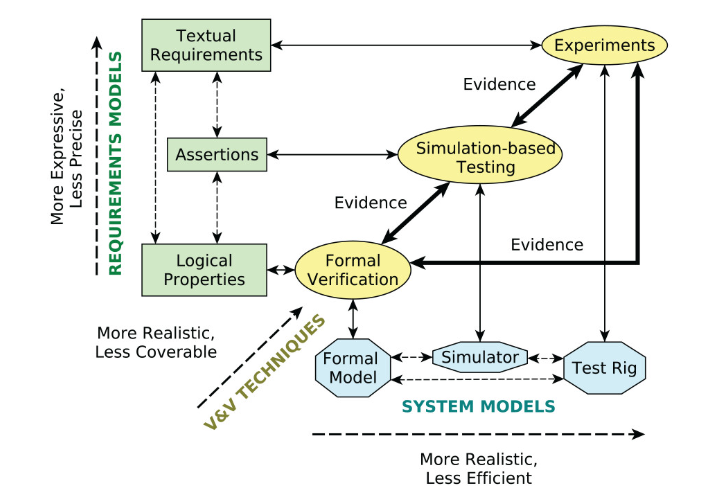
\includegraphics[width=0.8\linewidth]{pictures/FisherFigure.png}
    \caption{An overview of validation and verification (V\&V) techniques. Figure taken from \cite{VandVpaper}.}
    \label{fig:ConsensusGroupsFromArticle}
\end{figure}
%Måske skal det her kortes ned og flettes ind i nedenstående punkt?
In this project, we will be using the modeling tool UPPAAL to model and analyse a swarm robotics algorithm using simulation and statistical model checking. While we aspired to do formal verification as a way to guarantee concrete behaviour of the algorithm, we abandoned this pursuit due to a multitude of reasons. For one, we quickly realized that the state space of our model of the chosen algorithm is very large. This immediately complicates formal verification as the process of exhaustively checking the state space becomes expansive. Secondly, we observed that the interesting, emergent behaviours of our model were not prevalent until larger swarm sizes, further impeding our ability to do relevant formal verification. For these reasons, we elected to pursue model simulations and statistical model checking. We elaborate on this further in section \ref{sec:methodology}.

\subsection{Modeling, verification and properties}

Model checking is a verification technique for assessing* whether a system satisfies properties obtained from its specification \parencite[p. 3]{Baier_Katoen_2008}. Specifically, model checking can be defined as the automated technique of systematically checking whether a given formal property holds for a given finite-state model of a system \parencite[p. 11]{Baier_Katoen_2008}. As can be seen from this definition, model checking involves a number of activities*.* 

First of all, in model checking a \textit{model} is constructed from the system, that is, a formal unambiguous representation of the possible behavior of the given system \parencite[p. 12]{Baier_Katoen_2008}. Whereas the concrete formalism of the model depends on the modelling tool used\footnote{See section 4 for the case of UPPAAL}, the model is usually comprised of a number of states/locations, denoting evaluations of variables etc., and possible transitions between those states, denoting changes in the system (\parencite[p. 12]{Baier_Katoen_2008}). These models are derived from the specification of the system and can be more or less implementation-independent. 

The \textit{properties} to check the system against are also expressed formally in a property specification language, e.g. a linear-temporal logic, expressing propositions about possible behaviour over time, such as "It is always the case that \textit{p} eventually holds" \parencite[p. 12]{Baier_Katoen_2008}.  

Lastly these properties are \textit{checked systematically} on the model. This is done algorithmically by the model checking tool, analysing possible behaviors of the model \parencite[pp. 7, 13]{Baier_Katoen_2008}.

There are a number of motivating factors for using model checking for verification. First, model checking requires stating the system and its specification in formal terms. This encourages that the system under test is understood and expressed unambiguously early on, which can often highlight ambiguities in the specification of the system \parencite[p. 7]{Baier_Katoen_2008}. This has proved useful in our project, as we have found many ambiguities in the specification of the modeled swarm algorithm, many of them early on. We will discuss these later.* 

Another motivation for using model checking is that the system can be modeled and checked against properties at design stage and independent of implementation details. Ideally the model contains only details necessary for property-checking and abstracts away implementation- and hardware specific details. This makes analysis of the system easier, and the model can, afterwards, serve as a guiding blue-print for subsequent (possibly many) implementations of the system \parencite[pp. 145-146]{Brambilla}. This is beneficial in the case of our project, as it makes it possible for us to check properties for the swarm algorithm in a general way before deciding on a specific platform for implementing it.

However, model checking still does not eliminate the potential for errors: The verification is only as good as the model of the system, that is, if the model faithfully represents the system (\cite[pp. 145-146]{Brambilla}, \cite[p. 8]{Baier_Katoen_2008}). As such, we are aware that our model itself can present a source of error, if not done carefully. To account for this, we have made a number of formal properties expressing expected behavior of the system, which the system can be checked against as a sanity check. 


%(evt. lidt om formal verification vs. smc)
%(evt.: lack of fault-injection/faulty systems?)**

%%%Maybe first part should be later in report???***

\subsection{Statistical model checking}
%%Fix citationer!!!
We are using the model-checking tool UPPAAL 5.0 \footnote{\url{https://uppaal.org/}} for modelling and property-checking the swarm algorithm. Especially, we are using features from UPPAAL's statistical model-checker, UPPAAL SMC \footnote{\url{https://uppaal.org/features/}}. Contrary to "classical" UPPAAL, UPPAAL SMC does not \textit{verify} properties as such, by exhausting the entire state space of the model in question. Rather it runs simulations of the system, and uses various statistical results to determine whether a given property is satisfied with a certain degree of confidence \parencite[p. 398]{UPPAALSMC}. This \textit{slacking} of the coverage of model-checking allows utilizing more modelling-features such as floating-point-operations and arbitrary clock-rates*, and it makes model-checking much faster*. As such UPPAAL SMC trades off exhaustive analysis for the feasibility of simulating and checking systems with a much larger state-space. 

%% \textbf{(evt. kort afsnit om model, hvor det viste sig urealistisk at lave symbolsk analyse)***}

We also considered using PRISM\footnote{\url{https://www.prismmodelchecker.org/}} for our model checking. PRISM is a popular tool for modeling systems showing probabilistic behaviour (ref*). But while PRISM also supports statistical model-checking, we found that UPPAAL provided better and more intuitive support for certain modeling features (floating-point-operations, data-structures, functions and initialization of processes*). And in general, we deem the statistical checking features in UPPAAL SMC sufficient for our purpose.

\subsubsection{Basic modelling formalism}

In UPPAAL a system comprises a network of timed automata, each functioning* in parallel \parencite[for a formal definition see:][]{UPPAALTutorial}. A timed automata consists, similar to a finite-state-machine, of a number of locations\footnote{We (as well as UPPAAL) use the term 'location' rather than 'state' as to not conflate it with the state of the automata and the system}*, and a number of edges*. Exactly one of these locations is the \textit{initial} location, meaning that the automaton will always start in that location \url{https://docs.uppaal.org/language-reference/system-description/templates/locations/}. Additionally, an automata can own a number of local variables.  Each edge can have a number of actions (concretely called "updates" in UPPAAL) associated to them, which are performed when enabling the edge, as well a number of guards-conditions required to enable the edge. 

The automaton is \textit{timed} in the sense that it can also contain a number of clocks, the values of which is constrained by invariants on locations. All clocks progresses synchronously and evaluates to a real number at each given moment.* However, individual clocks can be stopped or reset, and alternative clock rates can be specified.*

Automatons can also use globally defined channels for synchronizations. We found that modeling synchronizations through functions rather than channels made our model easier to understand.*

A \textit{state} in a timed automaton is defined by the location, evaluation of its variables and evaluation of its clocks. The state of the entire system is defined by the states of all timed automatons with the addition of evaluations of \textit{globally} defined variables and clocks. A transition, changing the state of the system, can happen in two ways: 1) an automaton enables an edge at a given time, triggering any updates associated with the edge, or 2) an automaton performs a \textit{delay-transition}, staying at it's current location for a given duration $d\in 
\mathds{R}_{+}$, constrained by given invariants. The change is chosen non-deterministically. 

\subsubsection{Making a system in UPPAAL}

In practice, a system made in UPPAAL comprises a number of templates for instantiating timed automatons, global variable declarations, local declarations for instances of each template, and a system declaration for instantiating a number of automatons. An example can be seen in fig \ref{fig:ex-system}, which we will now consider.


\begin{figure}[!b]
    \centering
    \begin{subfigure}{0.90\textwidth}
        \centering
    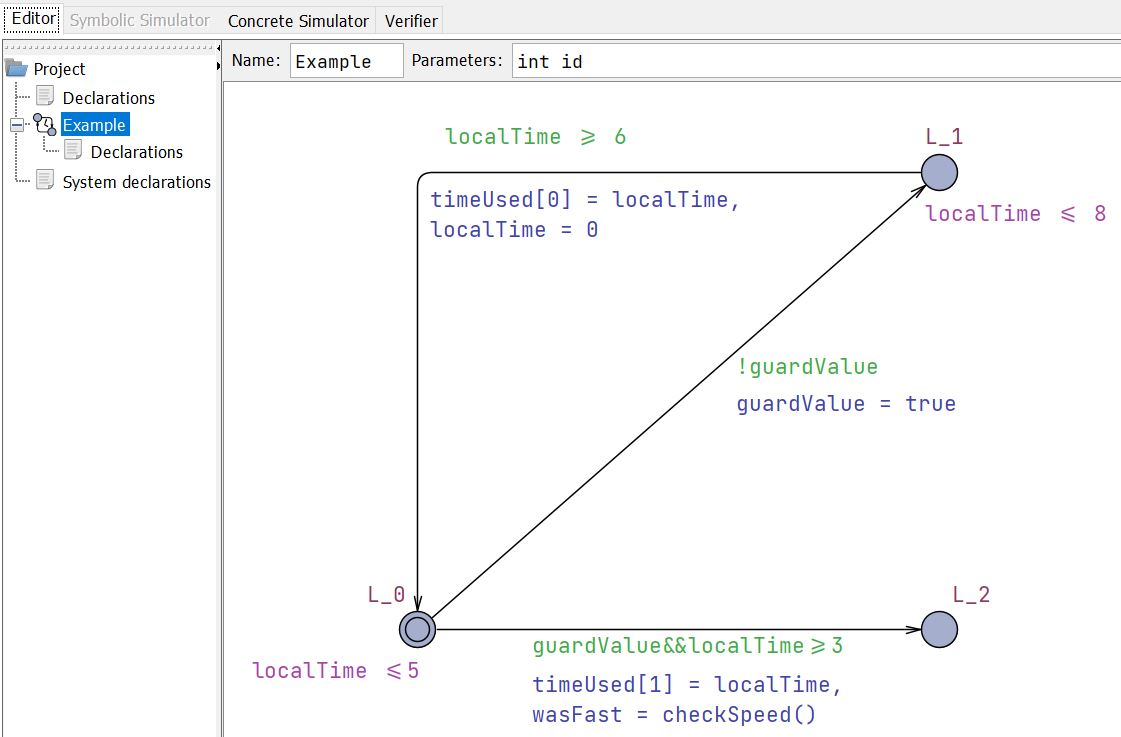
\includegraphics[width=\textwidth]{pictures/example_model_timed.JPG}
    \caption{Template for automata}
    \label{fig:ex-template}
    \end{subfigure}
     
    \medskip
     
    \begin{subfigure}{0.90\textwidth}
         \centering
    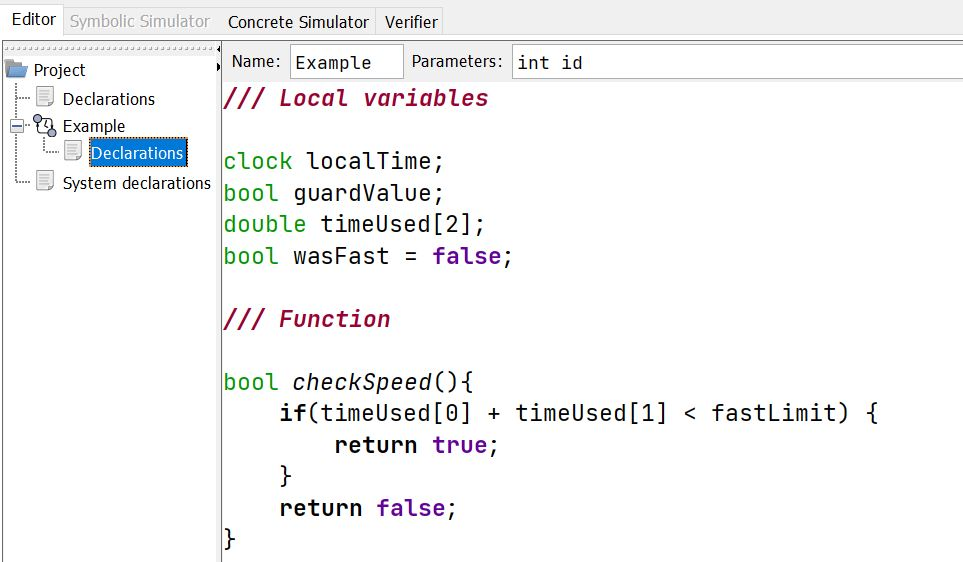
\includegraphics[width=\textwidth]{pictures/Local_declarations_example.JPG}
    \caption{Local declarations}
    \label{fig:ex-local-declarations}
    \end{subfigure}
    
    \caption{Example system in UPPAAL}
\end{figure}

\begin{figure}[ht]\ContinuedFloat
    \centering
    \begin{subfigure}{0.90\textwidth}
         \centering
    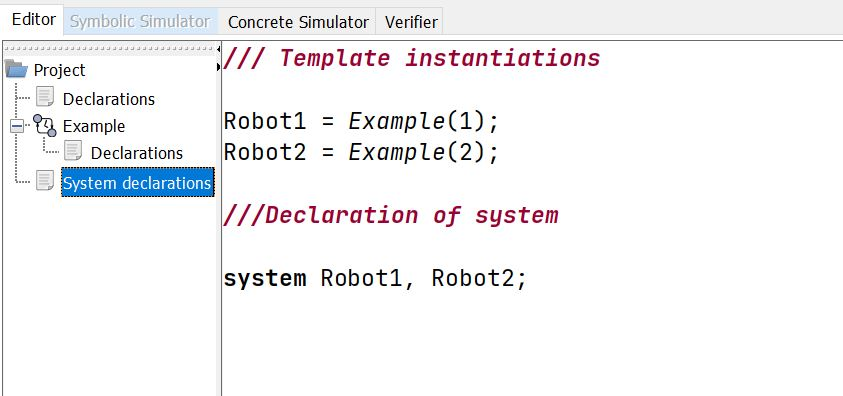
\includegraphics[width=\textwidth]{pictures/System_declaration_example.JPG}
    \caption{System declaration}
    \label{fig:ex-system-declaration}
    \end{subfigure}
     
    \medskip
     
    \begin{subfigure}{0.90\textwidth}
    \centering    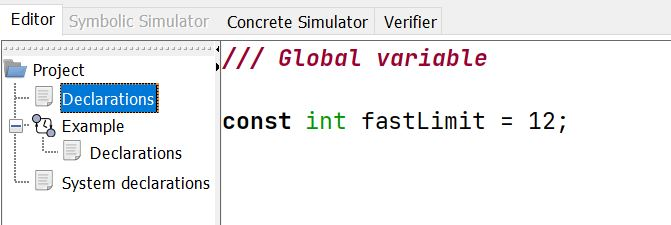
\includegraphics[width=\textwidth]{pictures/global declarations_example.JPG}
    \caption{Global declarations}
    \label{fig:ex-global-declarations}
    \end{subfigure}
    
    \caption{Example system in UPPAAL (cont.)}
    \label{fig:ex-system}
\end{figure}

The global declaration of the system is placed in the "Declarations"-file. In this case (see figure \ref{fig:ex-global-declarations}) the system has just one such value, \verb|fastLimit|, which is a constant of type \verb|int| with value 12.

In this example, the system has just one template, called \verb|Example|. The template has a diagram-representation associated, as seen in fig \ref{fig:ex-template}. Also, indicated in the top, a number of parameters can be specified for the template, specifying arguments that must be given an instantiation of the template \parencite[p. 4]{UPPAALTutorial}. The \verb|Example|-template has just one parameter, \verb|id| of type \verb|int|.

The \verb|Example|-template also has a number of local variables and functions associated to it, as seen in \ref{fig:ex-local-declarations}. In this case, a clock, \verb|localTime|, two boolean values, \verb|guardValue| and \verb|wasFast|, and a size-2-array of type double, \verb|timeUsed[]|. Additionally \verb|Example| has a function, \verb|checkSpeed()|, associated.
%that can be called by \verb|Example|-instances

Looking at the diagram in \ref{fig:ex-system}, the \verb|Example|-template has three locations, denoted by the circles \verb|L_0|, \verb|L_1| and \verb|L_2|. The circle inside \verb|L_0| indicates that it is the initial location of the automaton. At \verb|L_0| and \verb|L_1| invariants are associated, written in purple, indicating bounds on for which interval of values of \verb|localTime| an automaton can be in said state. For example, the automaton can only be in state \verb|L_0| when \verb|localTime| $\in [0,5]$.

There are also a number of edges connecting the locations, indicated by arrows. Each of these edges has a guard associated to it, written in green, and one or more updates, written in blue and separated by ",". For example, the edge from \verb|L_0| to \verb|L_2|
can only be enabled, if \verb|guardValue| evaluates to true and \verb|localTime| exceeds 3. And when the edge is traversed, \verb|timeUsed[1]| is set to the value of \verb|localTime|, after which \verb|wasFast| is set to the value returned by calling \verb|checkSpeed|.
 
Putting all of the above together, an instance of the \verb|Example|-template, goes from \verb|L_0| to \verb|L_1|, back to \verb|L_0| and finally to \verb|L_2| with delays within the time-bound, recording the value of \verb|localTime| at the second and last enabled edge. At the last enabled edge, it is checked, using function \verb|checkSpeed|, whether total time used (stored in \verb|timeUsed|-array) exceeds the global limit \verb|fastLimit|, in which case \verb|wasFast| is set to true. This order of enabling edges is determined by the guards of each edge, which require the first edge to be taken, updating \verb|guardValue| to true, which then makes it possible enabling the edge from \verb|L_0| to \verb|L_2|, but not from \verb|L_0| to \verb|L_1|.

As seen in fig \ref{fig:ex-system-declaration} two instances of the \verb|Example|-template is made with parameters 1 and 2 associated to variables \verb|Robot1| and \verb|Robot2|, after which the system is declared with the \verb|system|-keyword, consisting of the two instances. 

\subsubsection{Statistical model checking}

In UPPAAL SMC these automatons are extended with a stochastic component, replacing non-determinable transitions with probabilistic ones. If a location has a time-invariant, an edge transition is chosen by uniform distribution within that time-constraint. Otherwise one can specify a delay by choosing a rate, $\lambda$ for an exponential distribution for the delay, $d$, with PDF $F(d)=\lambda e^{-\lambda d}$ \parencite[p. 398]{UPPAALSMC}.\footnote{See also: \url{https://docs.uppaal.org/language-reference/system-description/semantics/}} 

When more (possible) edges are present in a given location, a given edge will be enabled according to uniform distribution. Or one can assign each of $n$ edges from a location a given probability, $p_i \in [0,1]$, where $\sum_{i=1}^n p_i = 1 $. 

Applied to our previous example, a modified version of the \verb|Example|-template with this extension could look like \verb|ExampleSMC| in figure \ref{fig:ex-template-smc}.

\begin{figure}[h]
    \centering
    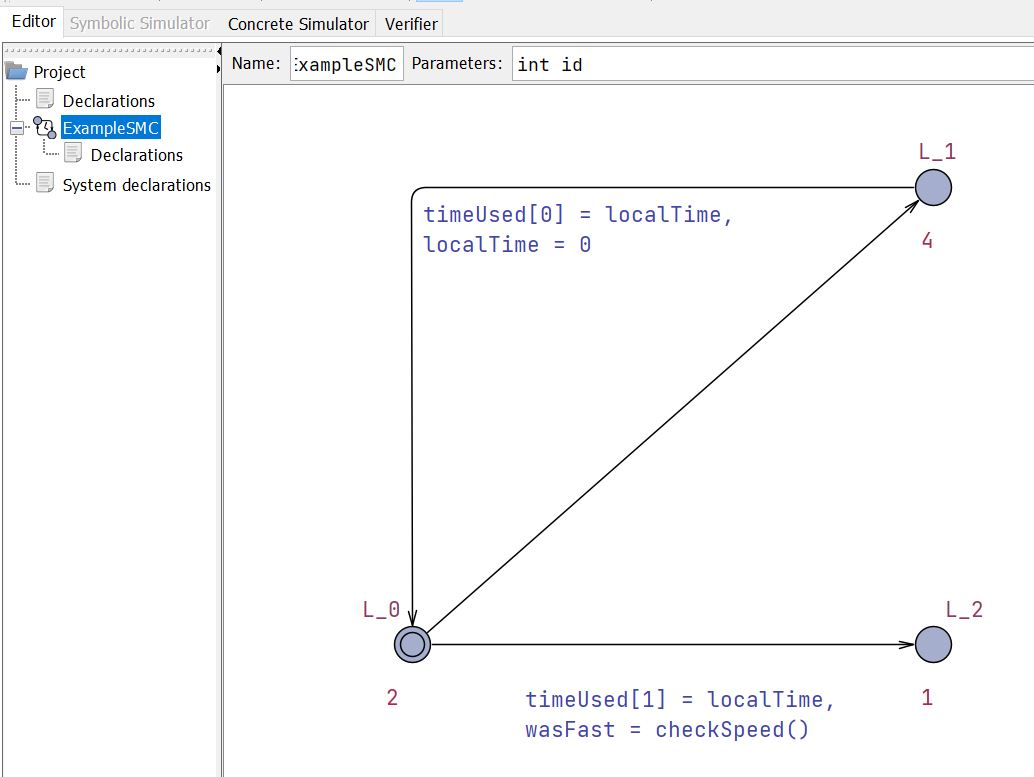
\includegraphics[width=0.90\linewidth]{pictures/example_model_smc.JPG}
    \caption{Example template with stochastic extension}
    \label{fig:ex-template-smc}
\end{figure}

In \verb|ExampleSMC| there are no guards on the edge from \verb|L_0| to \verb|L_1| nor the edge from \verb|L_0| to \verb|L_2|, so one of the edges will be randomly enabled with probability 0.5. Furthermore, instead of invariants, \verb|ExampleSMC| has exponential rates for the PDF of delays in each location, indicated by the brownish integers at each location.

Given this extension, it is possible to perform probabilistic queries on a model. In UPPAAL SMC these are expressed in MITL. These queries take on one of the following forms:

\begin{itemize}
    \item Simulate [\textit{bound}; \textit{N}]\{$expression_1,\, \dotsm \, , expression_n$\}
    \item E[\textit{bound}; \textit{N}]( min $|$ max :  \textit{expression} )
    \item Pr[\textit{bound}]($\phi$)
    \item Pr[\textit{bound}]($\phi$) $\geq$ \textit{probability}
    \item Pr[\textit{bound}$_1$]($\phi_1$) $\geq$ Pr[\textit{bound}$_2$]($\phi_2$)
    
\end{itemize}

Here $\phi$ is an MITL-formula* of the form [ ] $|<>$ \textit{expression}, where [ ] denotes "always holds" and $<>$ denotes "eventually holds".
%%\footnote{UPPAAL also supports full weighted MITL-expressions, but they have not been relevant for us} 
\textit{expression} denotes some state- or variable-based expression. \textit{bound} can be expressed in clock-values or number of edge-transitions.

To answer these queries, UPPAAL runs simulation of random runs of paths bounded by the length of the bounds. In the first two types of queries above, \textit{N} number of those runs are simulated, in which the values of the given expressions are monitored (their evaluation over time in the case of "Simulate"-queries and their expected minimum/maximum value in the case of E-queries). 

As such, if we want to track the value of \verb|localTime| over time in \verb|Robot1| over the course of 100 runs of length less than 10 time-units, we could check the query \verb|simulate [<=10;100]{Robot1.localTime}|. If we instead wanted the average maximum-value of \verb|localTime| for each of those runs, we could have checked the property \verb|E [<=10;100](max : Robot1.localTime)| against the system. 

In the last three cases a variable number of random, bounded runs are simulated, here modelled as Bernoulli random trials, where satisfying the given $\phi$ is equivalent to a success. A number of runs are simulated until, applying smc* algorithms (\cite[see:][]{UPPAALSMC}), the query can be answered with the desired confidence. For example, for checking the query Pr[bound]($\phi$), runs are repeatedly ran until the computed confidence interval has the a decired half-width $\epsilon$ and 
test-coverage $\alpha$.\footnote{\url{https://docs.uppaal.org/language-reference/query-semantics/smc_queries/ci_estimation/}} This mean that the running time of the statistical model checking depends on the desired level of confidence, and is otherwise linear on the bound-length of runs.

For example, if we want to check in the above system,  with confidence $\alpha=0.05$ and half-width $\epsilon=0.05$, the probability that \verb|wasFast| eventually evaluates to true for \verb|Robot1| within 2 time units, we can check the system against the property \verb|Pr[<=2](<>Robot1.wasFast)|. The value of the statistical operators \verb|\alpha| and \verb|\epsilon|, can be set under "Options->Statistical parameters" in the navigation bar. 

\begin{figure}[h]
    \centering
    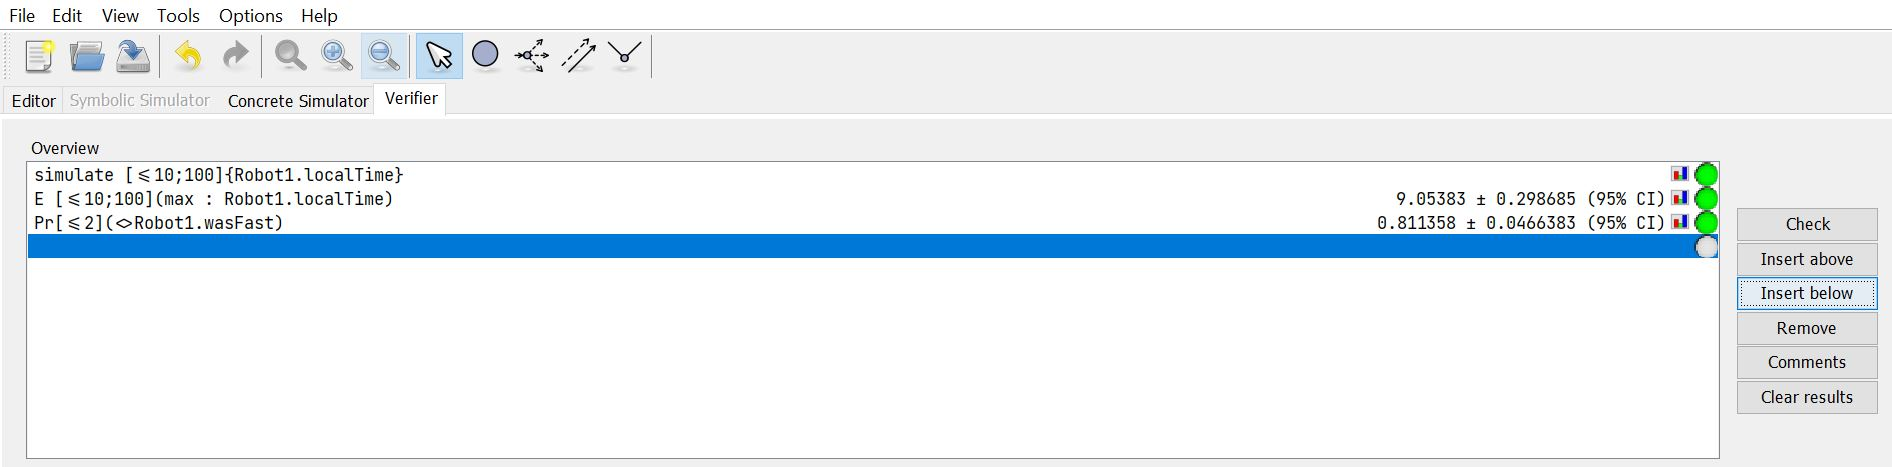
\includegraphics[width=1.0\linewidth]{pictures/properties_example.JPG}
    \caption{Example of probabilistic queries in Uppaal}
    \label{fig:ex-queries}
\end{figure}

As such, rather than exploring the state-space of the model, UPPAAL SMC confines itself to running a number of bounded simulations, which usually result in much faster running times for systems with huge state spaces.\footnote{\url{https://docs.uppaal.org/language-reference/query-semantics/smc_queries/ci_estimation/}}


 

\section{Lee-Liu Algorithm}
\subsection{Overview of algorithm}
As previously mentioned, our research project and UPPAAL model are based on the work by Yang Liu and Kiju Lee \parencite{AlgorithmPaper}. The article describes an algorithm for reaching a consensus in a decision-making process between an arbitrarily large swarm of independent, autonomous robots or agents that work together to accomplish some task. The algorithm was selected because it poses an interesting challenge in modeling the communication between agents, and because it suggests a number of experimentally decided metrics for how the algorithm should work. These metrics are useful for us to compare against our own model implementation.

The authors establish the following constraints on the algorithm (p. 3):
\begin{itemize}
\item Individual robots are primitive with limited sensing, communication, and processing capabilities.
\item Communication in the swarm is local; each robot can communicate only with nearby robots within the communication range. Robots within range will be referred to as neighbors for the rest of this report.
\item Robots have no temporal memory (i.e. no log of history data) and function like finite state machines.
\end{itemize}
We also note three assumptions:
\begin{itemize}
    \item The topology of the network will not change during the decision-making process.
    \item Robots have perfect and consistent communication among their neighbors.
    \item Robots are assumed to be somewhat globally synchronized, as the network is evaluated in terms of iterations. 
\end{itemize}

In summary, the algorithm works as follows:
\begin{itemize}
    \item There are $m$ robots, identified by their index in the set $R$. The set of possible decisions, \textbf{Q}, contains the indices for \textit{n} different choices. 
    \item Each individual robot is initialized with a distribution of preferences for each possible choice, given as a probability mass function $P_k$ for robot $R_k$. Each robot exhibits a decision, which is the choice it has the highest preference towards. For example, if $n = 3$, $R_k$ may have the set of preferences $\{P_k(1) = 0.25, P_k(2) = 0.5, P_k(3) = 0.25\}$, and it will exhibit a decision of choice 2.
    \item A robot has a connection group, \textit{C}, which consists of all of its neighbors. The robot knows the IDs and preference distributions of its neighbours. 
    \item A robot has a consensus group, \textit{D}, which consists of the largest connected component of robots that share the same dominant preference. See figure 1 below. A robot knows the IDs, but not the preference distributions, of the members in its consensus group. 
    \item A robot continuously updates its preference distribution by exchanging information with its neighbours. A robot will update its preferences to align with the predominant opinion among its neighbours, especially if their consensus groups are large.
    \item As the algorithm runs, the robots will become more certain in their decisions and stabilize their preference distributions, as long as nothing new is introduced in the network.
    \item When all robots share the same dominant preference, the algorithm terminates.
\end{itemize}

\begin{figure}[H]
    \centering
    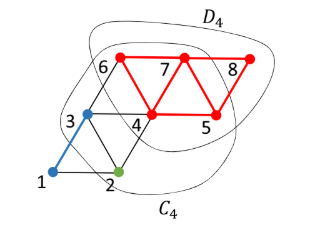
\includegraphics[width=0.5\linewidth]{pictures/Lee-Liu figure.png}
    \caption{"A network showing \(R_4\)'s local consensus group \(D_4\)
    and local connection group \(C_4\)" \parencite[Fig. 2]{AlgorithmPaper}.}
    \label{fig:ConsensusGroupsFromArticle}
\end{figure}

For a detailed explanation of the algorithm, we refer the reader to the original article \parencite{AlgorithmPaper}.
%For a more thorough explanation of the algorithm, the math and for an explicit use of the introduced formulas, see the original algorithm article and our UPPAAL implementation details.

\subsubsection{Interesting facets of the algorithm in modeling}

Apart from these assumptions that were explicitly stated in the original article, it is mentioned that the individual robot updates the members of its local consensus group. However, the provided explanation does not exhaustively address the issue that arises when one such change happens at a critical node in the local network of the consensus group. This, however, has become apparent as a result of our work in modelling the algorithm. 

To address this shortcoming, we present two different solutions: One makes use of our custom implementation of the Depth-first search algorithm\footnote{\url{(https://en.wikipedia.org/wiki/Depth-first_search)}} in UPPAAL to scan a global structure of the existing consensus groups, and thus finding their size, during every exchange of information between the individual robots. This approach adheres to the assumption of perfect local knowledge of the agents, but fails to adhere to the constraint of local communication. To rectify this issue, we present a second solution that follows more realistically the intended scenario - that the individual robots are indeed only able to communicate with their neighbours, and as such must use other means to address the predicament of figuring out the size of its local consensus group at any given time. This comes at a cost in convergence time, which we will discuss in later sections.
The authors of the article specifically state that interesting new avenues of research for the algorithm includes improvements to the discovery and updating of local consensus groups, including possible changes to the algorithm. This notion has also informed our decision in developing the previously mentioned UPPAAL models.

\subsubsection{Expected behaviour and results}
Lee and Liu present a number of different expected outcomes of their algorithm, as well as some ideal and anticipated behaviour under different circumstances based on both theoretical estimations and simulations done in a python script. These expectations are important benchmarks for us to compare against our own findings in our UPPAAL implementation of the algorithm. Here, we list some of the findings that we will discuss further in the results section of this paper.
\begin{enumerate}
    \item The network always reaches a consensus.
\end{enumerate}
This property of the algorithm serves as an important sanity check for us to determine that the model acts as intended. It is also the first property that we will check with our modeling tool.
\begin{enumerate}
    \setcounter{enumi}{1}
    \item The convergence rate is moderately correlated with network dependency.
\end{enumerate}
Network dependency is a term coined by Lee and Liu in the research article. Network dependency denotes the importance of the most critical node on maintaining the network connectivity \parencite[page 6]{AlgorithmPaper}. To facilitate testing the properties, we have coded a model generation tool in python that can also determine the network dependency value of the networks we use in simulation. We elaborate on this in section \ref{subsec:GG}.
\begin{enumerate}
    \setcounter{enumi}{2}
    \item The number of iterations needed to reach consensus is positively correlated with network size \textit{m} and the number of decisions \textit{n}.
\end{enumerate}
Larger networks and networks with a larger decision space take longer to correlate. We expect to see similar behaviour in our UPPAAL implementation.
Next follow a number of tests that we will try to replicate in our model, although the results are somewhat difficult to exactly reproduce, as they are based on randomly generated networks and their specific topologies.
\begin{enumerate}
    \setcounter{enumi}{3}
    \item The network converges significantly faster when seeded. The size of the seeding group and its placement in the network significantly affects this property.
\end{enumerate}
With 10 seed robots, a network of a 100 robots exhibits a 53\% convergence rate towards the dominant opinion of the seed robots. We will create similar trials to see if we can observe similar behaviour in our model.

\subsection{Graph Generation}
\label{subsec:GG}
For the purposes of testing and verifying their algorithm, Lee and Liu use a number of randomly generated networks. These networks have certain characteristics and properties that are relevant for the metrics of the algorithm. First, the networks are generated with a specific amount of robots \textit{m} and opinions \textit{n}. Second, all robots in the network have a maximum of 6 neighbours. This forms the equilateral triangle grids that is shown in the figures of the algorithm paper. Lastly, these graphs are each associated with a specific value of the previously mentioned \textit{network dependency}, a descriptor of the importance of the most critical nodes in maintaining connectivity in the network \parencite{AlgorithmPaper}. To stay as truthful to the original article as possible, we created a graph tool in python using NetworkX and Matplotlib \parencite{Hunter:2007, SciPyProceedings_11}. The code for this tool can be found in the link in the references \parencite{GraphTool} or in the appendix. We leverage this tool to create semi-random graphs from set values of \textit{n} and \textit{m}. The tool can subsequently calculate the network dependency of the graphs and draw visual representations of the generated networks. The tool also creates a direct string-representation of the network that can be copied into UPPAAL to recreate the same exact network.

\section{Methodology and Tools}
\label{sec:methodology}

\subsection{Modeling/tool methodology}

\begin{itemize}
    \item Use of time
    \item Use of syncronization in UPPAAL
    \item ...
\end{itemize}

\section{UPPAAL Model Implementation}

\subsection{Priorities and design decisions}

The problem of modeling an algorithm requires first identifyung those aspects of the algorithm that are of relevant for verification, and then simplifying and abstracting as much as possible while representing those interesting aspects faithfully.

In our case, considering the research questions, we are interested in the global state of the network, specifically the notion of iterations as a measure of running time.

We also considered different levels off abstraction in modeling, in part to explore the possibilities and limitations of modeling using probabilistic timed automata.

Finally, we prioritized respecting the constraints of the algorithm, specifically that robots should only have local information. We examined whether the process of transmitting local knowledge across the graph would introduce subtle changes to the theoretical behavior of the algorithm.
As we did not have a concrete implementation of the algorithm, we were interested in how much of a challenge it was to respect these constraints.

As a result the model represents a quite faithful simulation of the robots interactions as described in the paper. However, this required us to make a few implementation decisions of note that were left under-specified by the original authors.

This design decision introduced additional steps in the modeling process, as it requires modeling a communication algorithm, which in turn required additional debugging, implementation and verification steps.

As we are interested in the state of the network as a whole, we abstract away the concrete communication between robots. Instead, we simulate communication limits using a mask for each robot over global arrays indexed by the id of each robot. This mask is called \texttt{C}, and determines the network by describing local connection group for each robot. Following is an example og how a network of three robots in a line would look like:

\begin{verbatim}
bool C[3][3] = {{false, true, false},
                {true, false, true},
                {false, true, false}}
\end{verbatim}

This means that all information that a robot may request of a neighbor is available to be read without modeling concrete communication between those robots.

\subsection{Overview of model}

In our model, each robot is a process with an ID and five possible locations, including an initial and a terminal location.

The network can have either a completely random distribution of initial preferences, or it can be random with a number of seeded robots.
The number of seeded robots are controlled with the constant \texttt{SEEDNUM}, and the robots with a smaller id value get 100\% preference towards choice 0. This corresponds to Lie \& Lee's use of seed robots (section 3.4).
Though they do not specify the exact preference distribution given to seed robots, our results match theirs (see results section).

At location \texttt{PreferencesUpdated}, the robot has updated their preferences and their exhibited decision. At location \texttt{FindingDecisionGroup}, the robot is in the process of determining its consensus group $D$. At location \texttt{AwaitingNeighbors} the robot either terminates (if a global consensus has been found) or it moves on to a new iteration of updating its preferences (by traversing the edge to \texttt{PreferencesUpdated}).

\begin{figure}[H]
    \centering
    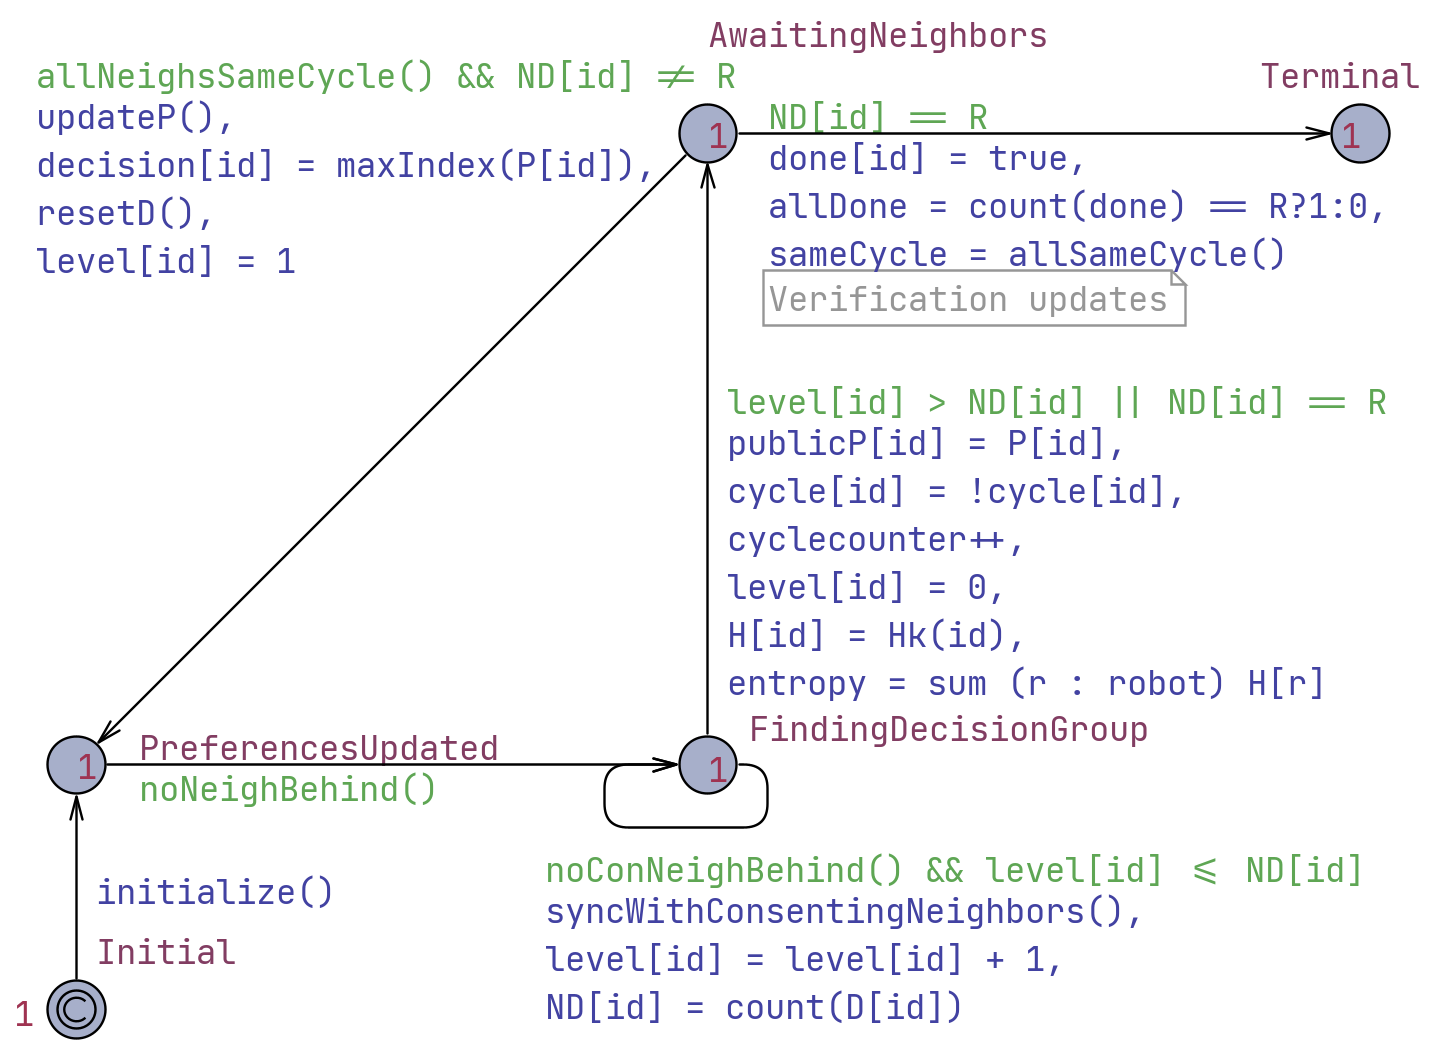
\includegraphics[width=\linewidth]{pictures/Model screenshot 2025-05-11.png}
    \caption{The Robot template in UPPAAL. Besides variable and function declarations, the system consists of $m$ instantiations of this state machine unique id values. Each state is named (in brown, capitalized), and has a rate of exponential of 1. Each edge transition has a guard statement (boolean expression) and a comma-separated sequence of assignments and method calls. Guard statements are in green and appear above assignments. They are placed as a block close to the edge they guard.}
    \label{fig:model}
\end{figure}

The edge from \texttt{Initial} to \texttt{PreferencesUpdated} directly corresponds to the initialization of the algorithm (section 2.1).
The edge from \texttt{AwaitingNeighbors} to \texttt{PreferencesUpdated} corresponds to both (section 2.2) preference updating via local interaction and (section 2.3) internal processing for decision uncertainty reduction.

All the edges leading to or originating in \texttt{FindingDecisionGroup} are needed to update the robots' local understanding of their consensus group, which is not specified as a separate step in the algorithm, but which requires a separate step in the model to preserve the constraint of local communication. We describe the algorithm for calculating consensus groups below.

\begin{table}
\begin{center}
\begin{tabular}{ lll } 
\hline
Code & Algorithm & Meaning \\
\hline
\texttt{D[id]} & $D_k$ & Consensus group for robot \texttt{id} / $k$\\ 
neighbors, or \texttt{C[id]} & $C_k$ & The connection group for robot \texttt{id} / $k$\\ 
\texttt{ND[id]} & $N_k$ & Size of consensus group for robot \texttt{id} / $k$\\ 
\texttt{P[id][j]} & $P_k(j)$ & Robot \texttt{id} / $k$'s preference toward decision $j$ \\
\texttt{decision[id]} & exhibited decision & The highest preference value of robot \texttt{id} \\
\texttt{R} & $m$ & Number of robots in system. \\
\texttt{Q} & $n$ & Number of decisions \\
cycle & iteration & A full update of preferences. \\
\texttt{EMPIRICAL} & $\lambda_T$ & The empirical threshold value convergence\\
\texttt{s[j]} & $s(j)$ & The rank of choice j for a given robot.\\
\texttt{Hk()} & $H_k$ & (section 3.1) Entropy value for robot $k$\\
\texttt{entropy} & $\sum H_k $ & Total entropy of system\\
\texttt{updateP()} & $P_k$ & Eq. 1. Include uncertainty reduction if relevant. \\
\texttt{divergence()} & $\lambda_k$ & Eq. 2. The degree of divergence for robot k\\
\texttt{accConvergence()} & $P^{new}_k$ & Eq. 3. The method normalizes the new values.\\
\texttt{L(s[j], Ll, Lu)} & $\mathscr{L}(s(j))$ & Eq. 4. The linear multiplier for choice $j$.\\
\hline
\end{tabular}
\caption{Explanation and translation of coding variables to algorithm terminology}
\label{tab:gloss}
\end{center}
\end{table}

\subsubsection{Timing and synchronization}

Because the paper did not specify any absolute or relative timing requirements, we decided not to give time invariants to locations, and rather uniformly give each location an exponential rate of 1. In our system, then, time is a proxy for the average number of edge traversals of the robots.

In terms of synchronization, the robot uses three local variables: the booleans \texttt{mayContinue} and \texttt{cycle[id]} and an integer \texttt{level[id]} bounded by the number of robots \texttt{R}.

\texttt{mayContinue} guards most edge traversals and is a product of the other sunchronization variables, depending on robot's current location.

\texttt{cycle[id]} represents the current cycle of the robot, relative to its neighbors. The cycle is flipped when traversing the edge between \texttt{FindingDecisionGroup} and \texttt{AwaitingNeighbors}. To continue from that location, all of a robots neighbors must be on the same cycle. Deadlocks are avoided because no robot will traverse a full cycle before all of its neighbors has exited \texttt{AwaitingNeighbors}, as they also have to synchronize at location \texttt{PreferencesUpdated}.

\texttt{level[id]} represents the progression of the robot within its current cycle, and is reset to 0 with each new cycle. Level 1 and above signifies that a robot has updated its preferences and exhibited decision. By waiting for all its neighbors to reach level 1 a robot ensures that it knows which neighbors exhibits the same decision (consents with) it, which is a precondition to determine its consensus group. 

When determining the consensus group, a robot continuously updates its consensus group to be the union of all its neighbors. This process is synchronized using levels, such that all information is guaranteed to travel throughout the consensus group withing \texttt{R} levels. We give a more thorough walkthrough of this algorithm below.

In total, local synchronization is quite strict, a robot waits for all its neighbors to reach a certain state twice within each cycle, and potentially waits for all consenting neighbors at each level between 1 and \texttt{R}. However, at a global level, we this model makes no assumptions about neither speed or interleaving of updates. There is no assumed global clock, and in a large network, at a given time before consensus is reached, robots may have completed quite different numbers of cycles, while in the end they will all have completed an equal number of cycles. 
This is interesting for two reasons: The loose global synchronization shows that the properties we test hold for networks without global coordination, and the strict local synchronization is part of the networks strategy to increase fairness.

\subsubsection{Fairness and atomic updates}

When considering the implicit assumption in the original article that robots are globally synchronized in iterations, we find that the specific synchronization policy influences the behavior of the algorithm.
A robot that reevaluates their preferences at a higher rate than its neighbors becomes more influenced by its neighbors than in reverse. Also, robots out of sync introduce possibilities of data consistency errors as robots request and update their preferences, and determine their consensus groups concurrently.
One way of solving this would be to have global synchronization with a predetermined order of updates for all robots, however as noted above, we were interested in respecting the requirement that robots do not communicate globally.

By using the above synchronization methods, we ensure that all robots complete the same number of preference updates, and that at any given time, a robot can at most be one update ahead or behind its neighbor. With no further modification, we would be left with the problem that the result of updating a robots preferences is influenced by the sequencing of when the robots in its connection group update their preferences.

We solve this by implementing a public / private distinction for the preferences. A robot updates its \texttt{P[id]} array by reading from each robot $r$ of its neighbors'  \texttt{publicP[r]} array. The  \texttt{publicP} arrays are updated when entering the \texttt{AwaitingNeighbors} location. In this way the updates to a robot and its neighbors preferences occur as if instantaneously from the perspective of a given robot.

\subsection{Algorithm for locally determining consensus group}

Since any change in exhibited decision in any robot can result in a drastic change in the consensus group of another robot, we consider the most transparent and faithful model to be one in which every robot recalculates its consensus group at each cycle.

The algorithm has three requirements: The consensus groups should be correct, it should not change the behavior of the algorithm and it should only use local information. Further, we want the process to not take too much time, and it should be as simple as possible so it is easy to analyze and reason about.

In our approach, each robot starts out by including only themselves in their decision group. Then all robots continuously pull decision group information from their connected consenting neighbors, and eventually, all robots will be aware of all members of their consensus group.

To synchronize this behavior, a robot is only allowed to pull information if no consenting neighbor is at a lower level than it. When it has pulled information, it increments its level and recalculates its local understanding of its consensus group size.
This ensures that all information will be travel across the consensus group. 
In the worst case, the information from one robot travels in a path including all other robots in the consensus group before reaching a final robot, and so the total number of levels gained required to be certain that all information has been gained is equal to the number of robots in the correct consensus group.
Because of this insight, we can reason that if a robots has a local understanding of its consensus group size $d$, and it has gained $d$ levels, then it is certain that it has found the correct consensus group.

An inductive reasoning of the above arguments goes as such: 

In the base case, where the correct $|D| = 1$, a robot initially believes $|localD| = 1$, which is correct. However, to be certain it is correct, the robot tries to pull information from its neighbors, does not find any new information, gains a level, and concludes that it is finished, since it has gained 1 level and has $|localD| = 1$. If $|D| = 2$, the robot must have found that out when asking its consenting neighbor, just as the consenting neighbor must have found that out when asking it. 

If $|D| = 3$, at least one robot must find out about both of its connected consenters in the first level, in which case it repeats for a few levels without learning anything new. If any robots do not find that out in the first level, they still must find one other robot and so have a $|localD| = 2$. In that case, they have still only gained one level so repeat the process once more. They must find out about the final robot in the next level, since they are connected to a robot that has found out about it.

Described another way, if a robot has $|localD| = d$ and is level $d-1$, it must pull information again. Then it either does not find anything new or does, in which case $|localD| = e$, $e > d$ and the robot must continue pulling until it is level $e-1$, at which point the scenario repeats.


\subsection{Verification of model}

While we are using the model to verify properties of the algorithm, we have also separately worked on verifying the quality of our model itself.

We made another model using depth-first search to determine the decision group sizes and simpler synchronization policies. 
The idea is to compare the behavior of those models. (DO WE FIND ANY DIFFERENCE IN BEHAVIOR?)

We have come up several test topologies of small networks. 
These include a minimally connected (a line) and a maximally connected network, a circular network and a randomly generated network.

The basic properties we check to see if the networks behave correctly are:

\begin{enumerate}
    \item All robots terminate in the same cycle and within a bounded time frame.
    \item The model-checker fails to find an example of a network that after a bounded time frame is not completed.
    \item The expected number of cycles and expected time before termination are measured as a sanity check to see if performance changes unexpectedly after changes to the network or to the model.
    \item The entropy is measured to show that entropy falls with a sufficiently high \texttt{empirical} value, and does not if \texttt{empirical} is 0.
    \item The chance of the consensus being decision 0 is measured, to make sure it corresponds to random chance for unseeded networks, and is high for seeded networks.
\end{enumerate}

See \ref{fig:properties} for the concrete syntax.

We have also continuously inspected concrete simulation traces to compare actual behavior with expected behavior.

Finally, we have used a few evaluation variables to construct basic verification queries to check in the statistical model checker.

\begin{figure}[H]
    \centering
    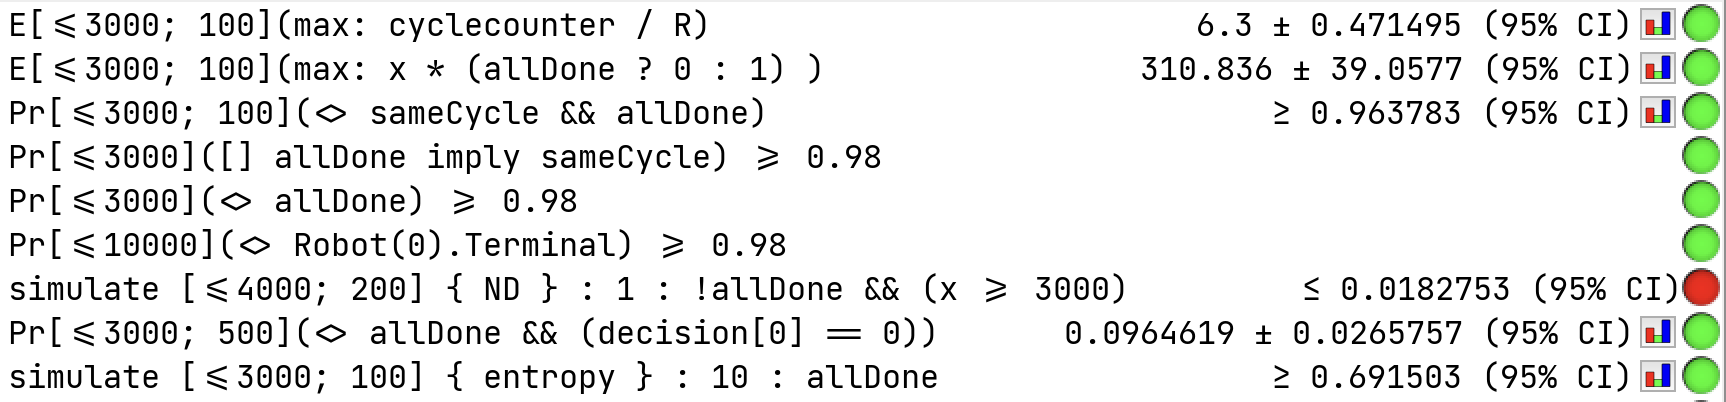
\includegraphics[width=\linewidth]{pictures/Properties.png}
    \caption{All properties checked to verify model.}
    \label{fig:properties}
\end{figure}

\subsubsection{Evaluation variables}

We have introduced five global variables to monitor properties of the algorithm.
\texttt{done[id]} reflects if a robot is in the terminal state. \texttt{allDone} reflects if all robots are in the terminal state. \texttt{sameCycle} reflects if all robots are in the same cycle after termination. \texttt{cyclecounter} counts the total times any robot has completed a cycle. If all robots end in the same cycle, then \texttt{cyclecounter / R} gives the number of (global) cycles before a consensus was reached.
\texttt{H} and \texttt{entropy} are measures of the global entropy in the system, derived using the formula in Liu \& Lee (section 3.2).

\subsubsection{Uncertain quality of convergence acceleration algorithm}

We have implemented the decision uncertainty reduction part of the original algorithm.
It relies on an "empirical threshhold value" (section 2.3) $\lambda_T$.
We took that implicitly to mean that the value should be determined by experiment based on how much of a performance improvement it produces in terms of cycles before a consensus is reached. However, we have not found a clear example of any value resulting in faster consensus times. We have tested with many different values in the range of 0.001 to 100.0, and conversely tend to see increased average cycles to reach consensus. We have even found very rare edge cases where circular topologies can end in a stalemate with two equally large and dominating consensus groups for large values of $\lambda_T$ ($>1$).
We are confused and concerned about this behavior. On the one hand, we may have implemented the algorithm incorrectly. We can of course not prove the absence of bugs, but also, the process itself is not fully specified in the original paper; It is not clear how the resulting values should be normalizes (which they have to by definition of $P_k()$ as a probability mass function), nor is it clear if the convergence acceleration should be added to the preference update process or replace it.

On the other hand, the behavior makes sense intuitively. If a network at some point starts containing multiple locally converged competing clusters (which happens easily in linear or circular topologies), they will become increasingly confident in their decision and so it is to be expected that more cycles will be required for one cluster to convince another.

We therefor also consider if this is intended behavior, because convergence acceleration improves some other metric than number of cycles till consensus. E.g. the authors point out convergence acceleration reduces discrete entropy. We might also consider that the process qualitatively improves results in a way not easily measurable.

This is an area we will continue to explore to find some more satisfactory answers.

\section{Results}
In the following, we present the results of testing various properties of our model in UPPAAL. Our findings are then compared to the results from the algorithm paper's experiments, which were originally conducted in a python script using Pygame \parencite{AlgorithmPaper}.

\subsection{Property testing}
\subsubsection{Sanity checks and alignment}
Before diving into the actual data, we designed a number of UPPAAL queries to test whether our system behaved as expected. These include queries such as \texttt{Pr[<=10000](<> allDone) >= 0.98}, which tests whether the robots all reach the terminal state within a large time bound, and \texttt{Pr[<=10000]([] allDone imply sameCycle) >= 0.98}, which determines whether all robots are in the same cycle when the robots reach the terminal state. Both of these return that the property holds, i.e. that this happens with probability $>98\%$. Even if this number is not technically a guarantee, UPPAAL has not been able to produce a counterexample in the thousands of runs that we have done. Our inspection of the algorithm and these tests align on the expectation that the robots should always reach a consensus and terminate, and that the robots are in the same cycle when this happens. Additionally, we created tests for assuring that the options in the decision space, Q, were equally likely to end up as the network consensus. With the query \texttt{Pr[<=30000; 1000](<> allDone \&\& (decision[0] == 0))} we were able to determine that no matter the size of Q, the probability of selecting decision 0 as the consensus was always $1/n$.
\newline
\newline
The Lee and Liu experiment with the effects of a number of various parameters, namely the network topology and size, and the number of decicision from which the robots can choose. In the following sections, we run similar tests to compare our model against the more idealized results from the original article \parencite{AlgorithmPaper}. We defer this comparison to section 8.


\subsubsection{Effects of network topology}
\begin{table}[h!]
\centering
\begin{tabular}{|l|c|c|c|}
\hline
\textbf{Topology Experiment} & \textbf{Network Size} & \textbf{Number of Options} & \boldmath$D_{\text{rel}}$ \\
\hline
Original (\cite{AlgorithmPaper}) & 30 robots     & 30 options   & 0.22 - 0.43 \\
\text{Our Experiment}    & \text{30 robots} & \text{30 options} & \text{0.22 - 0.43} \\
\hline
\end{tabular}
\caption{Comparison of experimental designs for testing the effects of network topology}
\label{tab:experiment-design}
\end{table}

For the effects of network topology, we copied all of the experiment parameters. However, since the networks are randomly generated, they are never going to be exact duplicates of the original networks.
Like Lee and Liu, we run each experiment for a 100 trials and post the average in the graph below. Our exact queries can be found in appendix A.

\begin{figure}[H]
    \centering
    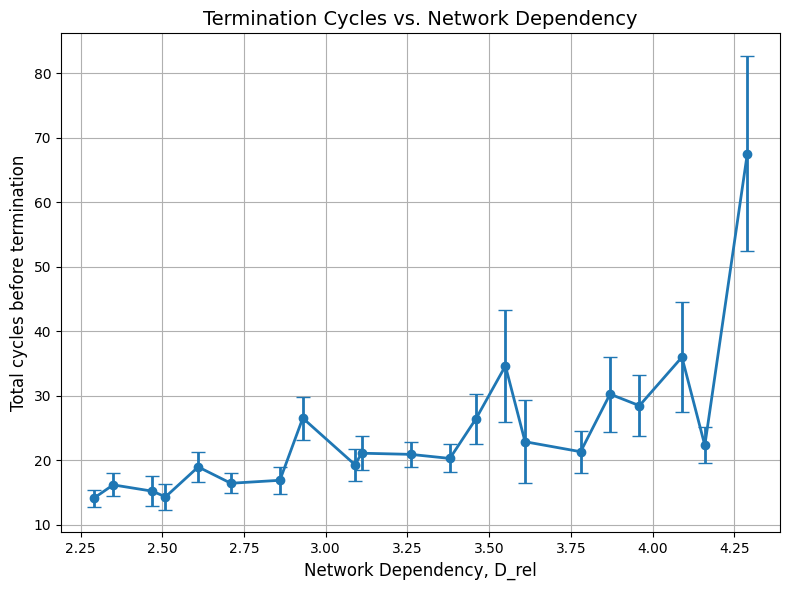
\includegraphics[width=0.9\linewidth]{pictures/DrelGraph.png}
    \caption{Results from experiments based on network dependency. The correlation between these variables have been found to have a Pearson value of 0.69}
    \label{fig:D_relResults}
\end{figure}

These variables are found to be moderately correlated with a Pearson value of 0.69 \parencite[page 1765]{pearson}. The results are statistically significant with P $<$ .00001.


\subsubsection{Effects of network size}
\begin{table}[h!]
\centering
\begin{tabular}{|l|c|c|c|}
\hline
\textbf{Network Size Experiment} & \textbf{Network Size} & \textbf{Number of Options} & \boldmath$D_{\text{rel}}$ \\
\hline
Original (\cite{AlgorithmPaper}) & 30 - 150 nodes     & 30 options   & 3.0 $\pm$ 0.1 \\
\text{Our Experiment}    & \text{5 - 50 nodes} & \text{30 options} & \text{3.0 $\pm$ 0.1} \\
\hline
\end{tabular}
\caption{Comparison of experimental designs for the effects of network size}
\label{tab:experiment-design}
\end{table}

For the effects of network size, we copied all of the experiment parameters as well as possible, but were forced to user smaller network sizes. This is imply due to how UPPAAL conducts the experiments, which becomes computationally heavy and unfeasible before the program crashes. The results, however, are still of interest.
Like before, we run each experiment for a 100 trials and post the average in the graph below. Our exact queries can be found in appendix A.

\begin{figure}[H]
    \centering
    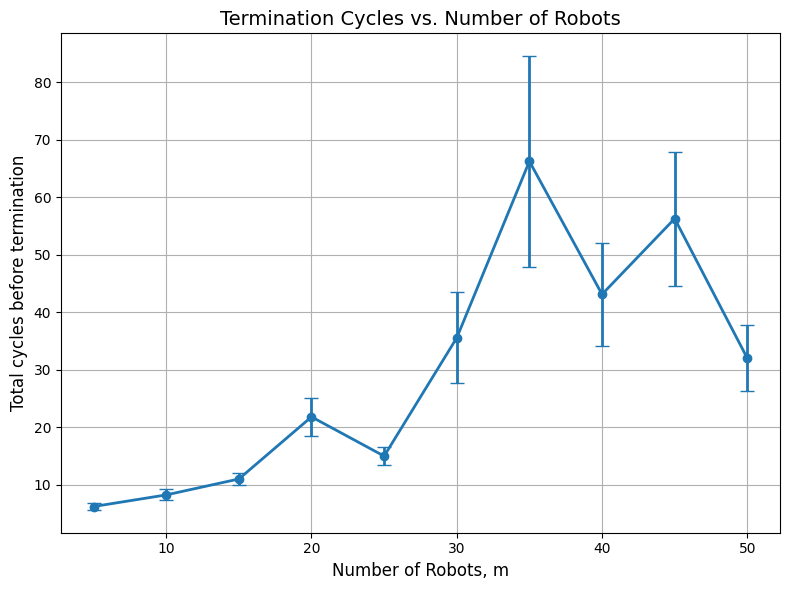
\includegraphics[width=0.9\linewidth]{pictures/RGraph.png}
    \caption{Results from experiments based on network size. The correlation between these variables have been found to have a Pearson value of 0.78}
    \label{fig:D_relResults}
\end{figure}

These variables are found to be strongly correlated with a Pearson value of 0.78 \parencite[page 1765]{pearson}. The results are statistically significant with P $<$ .00001.

\subsubsection{Effects of the size of the decision space}
\begin{table}[h!]
\centering
\begin{tabular}{|l|c|c|c|}
\hline
\textbf{Options Experiment} & \textbf{Network Size} & \textbf{Number of Options} & \boldmath$D_{\text{rel}}$ \\
\hline
Original (\cite{AlgorithmPaper}) & 30 nodes     & 10 - 300 options   & 2.672 \\
\text{Our Experiment}    & \text{30 nodes} & \text{10 - 300 options} & \text{2.675} \\
\hline
\end{tabular}
\caption{Comparison of experimental designs for the effects of option space size}
\label{tab:experiment-design}
\end{table}

For the effects of the size of the decision space, we copied all of the experiment parameters as well as possible, but due to the randomly generated networks, we had to choose a network with a 0.003 higher network dependency score. We expect that this small parameter will yield no significant change in the results.
Once again, we run each experiment for a 100 trials and post the average in the graph below. Our exact queries can be found in appendix A.

\begin{figure}[H]
    \centering
    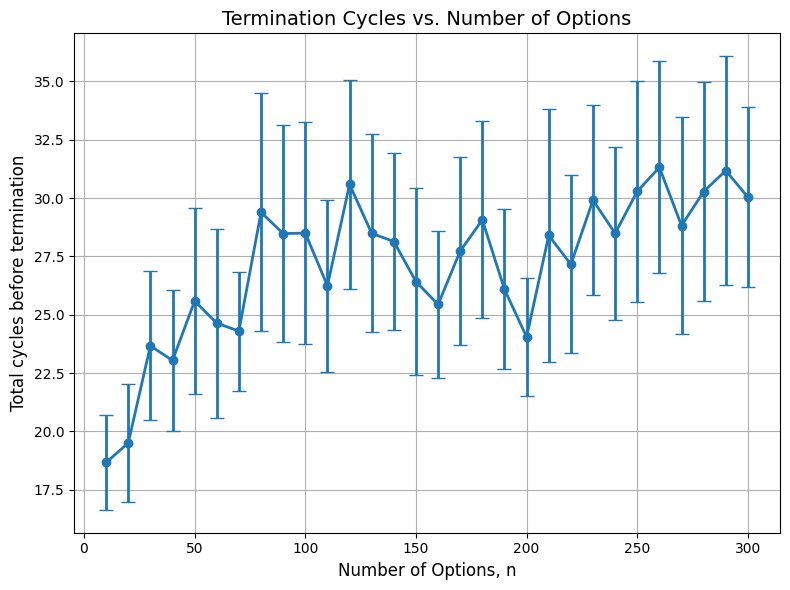
\includegraphics[width=0.9\linewidth]{pictures/QGraph.png}
    \caption{Results from experiments based on number of options. The correlation between these variables have been found to have a Pearson value of 0.73}
    \label{fig:D_relResults}
\end{figure}

These variables are found to be strongly correlated with a Pearson value of 0.73 \parencite[page 1765]{pearson}. The results are statistically significant with P $<$ .00001.

\subsubsection{Effects of the size of external interference}
Lee and Liu additionally run a number of experiments on the effects of seeding \parencite{AlgorithmPaper}. Seeding is meant as the act of predetermining the preferred decision of a number of robots. The effects of these seeds robots on the final outcome are then observed.
The details for the original experiment \parencite{AlgorithmPaper} are somewhat unclear. For example, there is no mention of the network dependency value of the networks or the size of the decision space. For our experiments, we will be using a randomly generated network of 30 robots with a network dependency value of 2.84. We set the number of options to 30, and predetermine the seed robots to exhibit a preference of 13\% for the first option at index 0, with the remaining options each having a 3\% preference. This spread can be largely influential, and no precedence is set in the original paper. Consequentially, the results should be interpreted as such.

\begin{figure}[H]
    \centering
    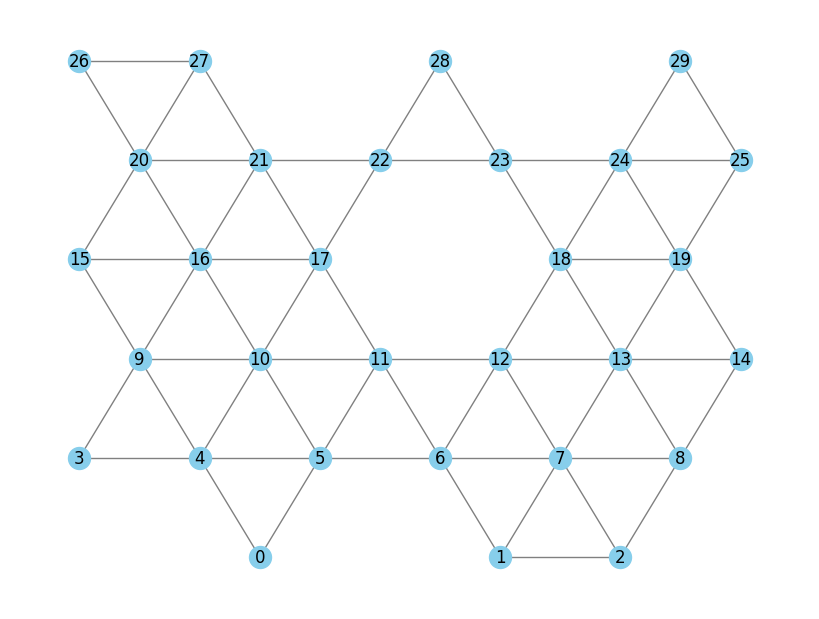
\includegraphics[width=0.9\linewidth]{pictures/30robs.png}
    \caption{Network of 30 robots for testing the effects of seeding.}
    \label{fig:D_relResults}
\end{figure}

We initially run our queries with no seeding. In the simulations, 3/100 runs end up with consenting on decision 0, and UPPAAL estimates the probability of selecting this decision to be between about $4.6\% \pm 4\%$. This is all in line with the expected value of $1/n$.  We then run a number of simulations, and get the following results.
\begin{figure}[H]
    \centering
    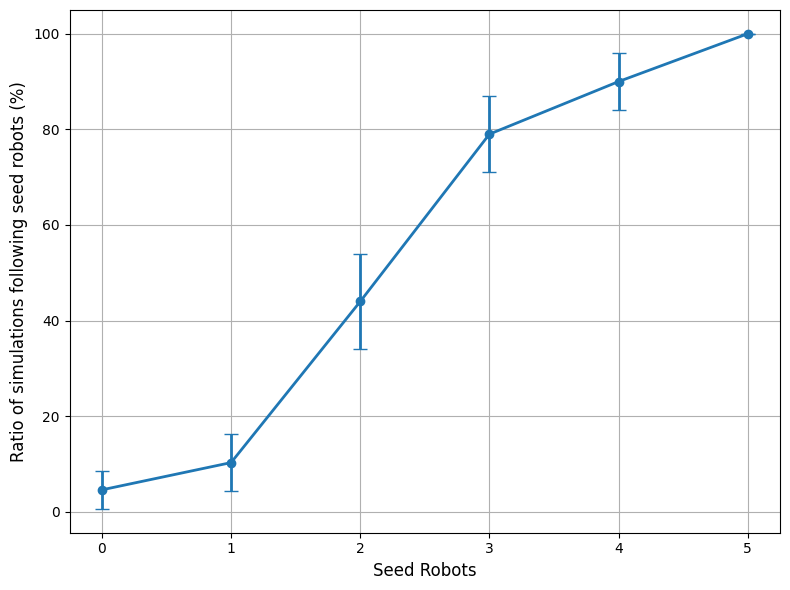
\includegraphics[width=0.9\linewidth]{pictures/SeedGraph.png}
    \caption{Effects of seeding on network consensus}
    \label{fig:D_relResults}
\end{figure}
From 5 seed robots and onward, the network always consents on the seeded decision.
%With a single seed robot, this probability jumps to $10.3\% \pm 6\%$, and at two seed robots, the probability leaps to $44\% \pm 10\%$. At three, $79\% \pm 8\%$, four, $90\% \pm 6\%$, at 5 robots and onward, the
\newline
We discuss these results in the following section.

\section{Reflections}

In this section, we reflect on the process and result of our work.
We note some potential improvements that could be made to our tool, UPPAAL, based on our experience as newcomers.
We also discuss a few underspecifiations and assumptions of the original paper.
We reflect on our approach to modeling, what stumbling blocks took a lot of time for us and what approach we have found to be helpful when modeling swarm robotics algorithms.
Finally, we consider how our work may be improved and built upon.

\subsection{UPPAAL as a modeling tool}

We have benefited greatly from UPPAALs support for types, functions and templates.
These features made it much easier for us to translate our existing programming knowledge into modeling work - which is even more enhanced by the C-like syntax.
UPPAAL is tool in development, and many useful and user-friendly features have been added during recent versions.
The graphical editor and simulator also make it easy to inspect the models behavior which greatly simplifies debugging.

However, UPPAAL suffers from outdated, lacking and at times incorrect documentation.
There are official documentation pages, but many specifications, language idioms, and behaviors are distributed over presentations and tutorial written over multiple decades and major software versions – there are even some rules in the language we have not found documented at all.
This leads to unexpected errors and inconsistent understanding of the rules of the language, which works counter to the purpose of formal verification.
The lacking documentation encourages a "try and see" approach to writing functions and models, where understanding is derived from empirical observation of the simulator.
Specifically for formal verification, it is crucial to be confident and exact in ones understanding of how changes to concrete syntax are translated into changes to the underlying model.
Therefore we argue that documentation is of special importance for a tool like UPPAAL.

Extending this observation, we found that while debugging and inspecting the model is easy, functions are not as well supported.
Because functions are called atomically during edge traversals in the simulator, there is no way of inspecting evaluation, which makes it hard to catch errors and verify behavior.

In our specific case, another limitation of the platform became apparent. 
UPPAAL has chosen to save systems as XML files and enforces a strict project structure.
This means that the entire project is saved as a single file, and is only comfortable to edit using UPPAALs own GUI editor.
Within the GUI, a project must have exactly one global declarations file, one declarations file per template, and one global declarations file.
Combined, this makes it cumbersome to collaborate on projects, as merge conflicts are inevitable and complex project cannot be broken down into components.
The ability to modularise a project in some way would make it possible to 

Finally, we note that UPPAAL currently has quite severe performance issues on newer MacOS machines that may stem from memory leaks.



\subsection{Correctness of our model}



\subsection{Realism of the algorithm}
\subsection{Relation between expected behaviour and model results}
In general, our results are very alike those presented in the algorithm article \parencite{AlgorithmPaper}. We find similar correlations between the various variables and the iterations needed for the network to converge and consent on a singular decision. In some cases, we have been unable to replicate the exact experiment setup that was used in the original work, but even with the approximate setups we get similar results. In terms of our fourth research question, we conclude that the numbers match exceedingly well. For both network dependency values, network size, options and external interference, the results from our synthesized automata model closely conform to the proposed values from the original article.
While network dependency value was found to correlate with the amount of iterations needed to finish a decision process, we have also found that it is not a perfect metric. Often during random tests and setup, we would encounter somewhat large variance in the iteration counts, even if two networks had the same network dependency value. This suggests that there are other factors of network topology that could be very relevant for how the algorithm performs, and certain structures that may cause long, unintended processes that impede and slow down the decision making process. We have not been able to pin down any other specific, significant structure, but we theorize that they exist, and leave the discovery to possible future work.


\section{Conclusion}


\newpage
\printbibliography

\newpage
\begin{appendices}
    \section{Queries}
    \label{ExampleLabel}
    \begin{figure}[H]
    \centering
    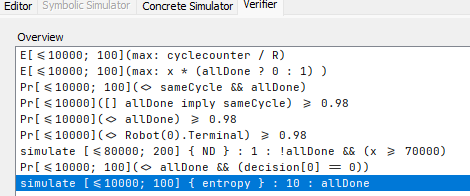
\includegraphics[width=\linewidth]{pictures/Queries.png}
    \label{fig:model}
\end{figure}
    \section{Networks}
    The networks can be found in the attached .txt files.
\end{appendices}
\end{document}
